% ---------
% --------
%!TEX TS-program = pdflatex
%!TEX encoding = UTF-8 Unicode
%!TEX spellcheck = English (Aspell)

\documentclass[11pt]{article}
\usepackage{lucy,handout,graphicx}
\usepackage{fourier-orns}
\usepackage{mathtools}
\usepackage[normalem]{ulem} % either use this (simple) or
\usepackage{tikz}

\def\Cdot{\mathbin{\text{\normalfont \textbullet}}}
\def\Sym#1{\texttt{\color{BrickRed}#1}}
\def\BlueSym#1{\textbf{\texttt{\color{RoyalBlue}#1}}}
\allowdisplaybreaks

\begin{document}

\begin{center}
\Large\textbf{CSCI 332, Fall 2026}%
\\
\LARGE\textbf{Homework 10 }%
\\[0.5ex]
\large Due Monday, November 9 Anywhere on Earth (6am Tuesday)
\end{center}

\bigskip
\hrule
\bigskip

\subsection*{Submission Requirements}
\begin{itemize}
    \item Type or clearly hand-write your solutions into a PDF format so that they are legible and professional. Submit your PDF on Gradescope. 
    \item Do not submit your first draft. Type or clearly re-write your solutions for your final submission. If your submission is not legible, we will ask you to resubmit.
    \item Use Gradescope to assign problems to the correct page(s) in your solution. If you do not do this correctly, we will ask you to resubmit.
\end{itemize}

\subsection*{Academic Integrity}

Remember, you may access \EMPH{any} resource in preparing your solution to the homework. However, you \EMPH{must}
\begin{itemize}
    \item write your solutions in your own words, and
    \item credit every resource you use (for example: ``Bob Smith helped me on
    this problem. He took this course at UM in Fall 2020''; ``I found a solution
    to a problem similar to this one in the lecture notes for a different
    course, found at this link: www.profzeno.com/agreatclass/lecture10''; ``Here is a link to the full transcript of my chat with ChatGPT about the problems on this HW''.)
    Ask if you need any clarifications about how to properly cite your sources!
\end{itemize}




\newpage
%----------------------------------------------------------------------
    
\headers{CSCI 332}{Homework 10 (due November 9)}{Fall 2026}


\begin{enumerate}
%\parindent 1.5em \itemsep 4ex plus 0.5fil

%----------------------------------------------------------------------

\item (0 points) List the resources you used for each problem in this homework. If you used no resources except
lecture notes and videos and the linked textbook, you can say ``none''. If you used
an AI tool, you should put a link to your full conversation here, and you must
use the
\href{https://umaal.org/files/teaching/csci332_fall2026/agents.md}{provided
prompt}
 to guide the AI to act
as a tutor, not an answer-provider.

You will be asked to resubmit your homework if this section is blank.

Remember that no matter what resources you consulted, you must write your solutions
\emph{in your own words}.

\item In Excel (and other spreadsheet programs), the values of cells
can be calculated as functions of the values of other cells. For example,
cell $A1$ can be assigned to have value $B1 + 1$. However, if cells reference
one another in a circular manner, then the values are undefined, and the program
must decide how to handle the error. In Excel, such circular references
produce an error:

\begin{center}
  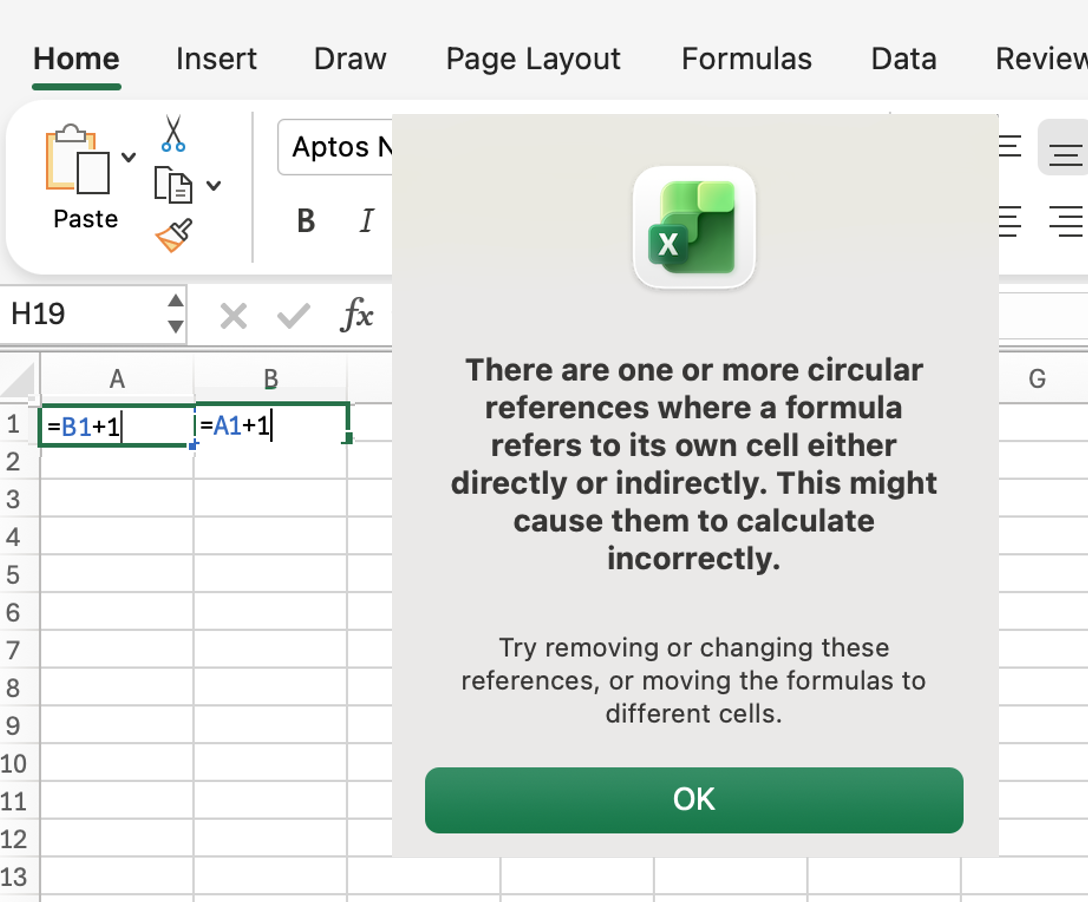
\includegraphics[width=.8\textwidth]{excel.png}
\end{center}

You are given the current state of a spreadsheet program as a
collection of $m$ strings representing the formulas in each cell.
Describe and analyze the runtime of an efficient algorithm to detect whether circular references
exist by reducing to a problem on a graph. You may write your answer in paragraph
form, as pseudocode, or however you prefer, but you will receive points for clearly addressing
each of the following: 

\begin{itemize}
\item What are the vertices?  What does each vertex represent?
\item What are the edges?  Are they directed or undirected?
\item If the vertices and/or edges have associated values, what are they?
\item \textbf{What is the precise relationship between your graph and the stated problem?}
\item What standard graph algorithm are you using to solve the problem?
\item What is the running time of your entire algorithm, \emph{including} the time to build the graph, \emph{as a function of the original input parameters}?
(Notice that $V$ and $E$ are \emph{not} parameters of the original problem.)
\end{itemize}
\end{enumerate}






%%%%%%%%%%%%%%%%%%%%
\end{document}
